\documentclass{article}
\usepackage{hyperref}
\usepackage{graphicx}
\title{Lab 14: \LaTeX{}}
\author{David Gardiner}
\date{\today}

\begin{document}

\maketitle

\section{Directions}
Your lab assignment today is to write the code to produce this document.
\begin{enumerate}
	\item First, write some code.
	\item Then, compile it with \texttt{pdflatex}.
	\item Check the pdf to see if it looks right.
	\item When you're done, submit your text file.
	\item Good luck on finals!
\end{enumerate}

\section{Text Formatting}
Sometimes, you \textit{may} want to \textbf{\underline{emphasize}} some text.

\section{Math}
Let $i^2 = -1$, or as you may recognize it, $i = \sqrt{-1}$.

Claim: $e^{\pi{i}} + 1 = 0$. Why on earth would this be true?

First, what does it mean for us to raise e to an imaginary power? Well, the 
Maclaurin series for $e^x$ might help us:

\begin{equation}
e^x = \sum_{k=0}^{\infty} \frac{x^k}{k!} = 1 + x + \frac{x^2}{2} +
\frac{x^3}{3!} + \frac{x^4}{4!} + \cdots
\end{equation}
(Hint: \textbackslash\texttt{cdots} makes a centered ellipsis.)

So, plug in $ix$:

\begin{equation}
e^{ix} = \sum_{k=0}^{\infty} \frac{i^kx^k}{k!} = 1 + ix + \frac{i^2x^2}{2} + 
\frac{i^3x^3}{3!} + \frac{i^4x^4}{4!} + \cdots
\end{equation}

\newpage 
Now we get to use our nice rule that says $i^2 = -1$:

\begin{equation}
e^{ix} = 1 + ix - \frac{x^2}{2} - \frac{ix^3}{3!} + \frac{x^4}{4!} +
\frac{ix^5}{5!} - \cdots
\end{equation}

Let's rearrange a little bit:

\begin{equation}
e^{ix} = \left(1 - \frac{x^2}{2} + \frac{x^4}{4!} - \cdots\right) - 
i\left(x - \frac{x^3}{3!} + \frac{x^5}{5!} - \cdots\right)
\end{equation}

If you put on your Macluarin series glasses and squint a bit, it turns out
that all this hootenanny reduces to

\begin{equation}
e^{ix} = \cos{x} + i\sin{x}
\end{equation}

And since $\cos{\pi} = -1$ and $\sin(\pi) = 0$, $e^{\pi{i}} = -1$.

\section{Figures}
If you like drawing pretty figures, you should look at 
\href{http://www.texample.net/tikz/examples/all/}{TikZ}.

If you want to read more about complex numbers and fractals, read
\url{http://acko.net/blog/how-to-fold-a-julia-fractal/}.

\begin{figure}[h]
  \caption{The complex plane!}

  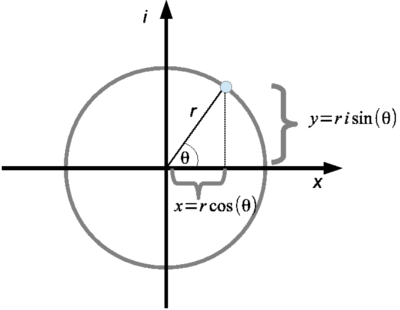
\includegraphics{complex.png}
\end{figure}

\end{document}
